% (c) 2012-2013 Claudio Carboncini - claudio.carboncini@gmail.com
% (c) 2012-2014 Dimitrios Vrettos - d.vrettos@gmail.com
% (c) 2015 Daniele Zambelli daniele.zambelli@gmail.com


\section{Esercizi}
\subsection{Esercizi dei singoli paragrafi}
% \subsubsection*{G.1 - Prime definizioni} 
\numnameref{sec:trigo_primedef}

\begin{esercizio}
\label{ese:G.1}
Completate la figura mettendo le opportune lettere ai vertici dei triangoli 
rettangoli assegnati e, applicando le definizioni, scrivete la formula
che permette di ricavare l'elemento incognito indicato con un punto 
interrogativo a partire dagli elementi noti indicati con una lettera.
\begin{center}
\begin{inaccessibleblock}[Alcuni triangoli rettangoli con dati un lato 
e un angolo acuto.]
 % (c) 2012 Dimitrios Vrettos - d.vrettos@gmail.com

\begin{tikzpicture}[x=10mm,y=10mm, font=\small]
  \coordinate (A) at (0,0);
  \coordinate (B) at ($(A)+(0:-2)$);
  \coordinate (C) at ($(A)+(90:3)$);

  \draw (C)--(A)--(B)--(C);

  \tkzMarkAngle[fill=LimeGreen, draw=black, size=.3](B,C,A)
  \tkzLabelAngle[pos=.6, font=\scriptsize](B,C,A){$\alpha$}
  \tkzLabelSegment[midway, right](A,C){$c$}
  \tkzLabelSegment[midway](B,C){?}

  \begin{scope}[xshift=10mm, yshift=-20mm]
    \coordinate (A) at (0,0);
    \coordinate (B) at ($(A)+(0:-2)$);
    \coordinate (C) at ($(A)+(90:3)$);

    \draw (C)--(A)--(B)--(C);

    \tkzMarkAngle[fill=LimeGreen, draw=black, size=.3](A,B,C)
    \tkzLabelAngle[pos=.6, font=\scriptsize](A,B,C){$\alpha$}
    \tkzLabelSegment[midway, right](A,C){?}
    \tkzLabelSegment[midway](B,C){$c$}
  \end{scope}

  \begin{scope}[xshift=15mm, yshift=12mm]
    \coordinate (A) at (0,0);
    \coordinate (B) at ($(A)+(0:4)$);
    \coordinate (C) at ($(A)+(60:2)$);

    \draw (C)--(A)--(B)--(C);

    \tkzMarkAngle[fill=LimeGreen, draw=black,size=.4](C,B,A)
    \tkzLabelAngle[pos=.6, font=\scriptsize](C,B,A){$\alpha$}
    \tkzLabelSegment[midway](B,C){?}
    \tkzLabelSegment[midway, below](B,A){$b$}
  \end{scope}

  \begin{scope}[xshift=15mm, yshift=-15mm]
    \coordinate (A) at (0,0);
    \coordinate (B) at ($(A)+(0:4)$);
    \coordinate (C) at ($(A)+(60:2)$);

    \draw (C)--(A)--(B)--(C);

    \tkzMarkAngle[fill=LimeGreen, draw=black,size=.4](B,A,C)
    \tkzLabelAngle[pos=.6, font=\scriptsize](B,A,C){$\alpha$}
    \tkzLabelSegment[midway](B,C){?}
    \tkzLabelSegment[midway](C,A){$c$}
  \end{scope}

  \begin{scope}[xshift=70mm, yshift=8mm, rotate=40]
    \coordinate (A) at (0,0);
    \coordinate (B) at ($(A)+(0:2)$);
    \coordinate (C) at ($(A)+(90:3)$);

    \draw (C)--(A)--(B)--(C);

    \tkzMarkAngle[fill=LimeGreen, draw=black, size=.4](A,C,B)
    \tkzLabelAngle[pos=.6, font=\scriptsize](A,C,B){$\alpha$}
    \tkzLabelSegment[midway, left](A,C){$c$}
    \tkzLabelSegment[midway,above](B,C){?}
  \end{scope}

  \begin{scope}[xshift=60mm, yshift=-20mm]
    \coordinate (A) at (0,0);
    \coordinate (B) at ($(A)+(0:2)$);
    \coordinate (C) at ($(A)+(90:3)$);

    \draw (C)--(A)--(B)--(C);

    \tkzMarkAngle[fill=LimeGreen, draw=black, size=.4](C,B,A)
    \tkzLabelAngle[pos=.6, font=\scriptsize](C,B,A){$\alpha$}
    \tkzLabelSegment[midway, left](A,C){$c$}
    \tkzLabelSegment[midway,below](B,A){?}
  \end{scope}
\end{tikzpicture}

\end{inaccessibleblock}
\end{center}
\end{esercizio}

% \subsubsection*{G.2 - Due identità fondamentali}
% \numnameref{sec:trigo_identita}

\begin{esercizio}
\label{ese:G.2}
Nel triangolo rettangolo~$ABC$ sappiamo che~$\sin \gamma =\frac{5}{7}$
Determinare le altre funzioni goniometriche dell'angolo~$\hat{\gamma}$ e quelle 
del suo complementare.
\end{esercizio}

% \subsubsection*{G.4 - Usare la calcolatrice}
% \numnameref{}

\begin{esercizio}
\label{ese:G.3}
Completare la tabella inserendo nelle caselle vuote misure di angoli acuti a 
piacere, approssimando alla quarta cifra decimale.
\begin{center}
\begin{tabular}{cccccccccc}
\toprule
angolo~$\hat{\alpha}$ & $0\grado$ & \ldots & $30\grado$ & \ldots & $45\grado$ & 
\ldots & $60\grado$ & \ldots & $90\grado$\\
\midrule
$\cos \alpha$ & & & & & & & & & \\
\bottomrule
\end{tabular}
\end{center}
\end{esercizio}

\begin{esercizio}
\label{ese:G.4}
Completare la tabella inserendo nelle caselle vuote misure di angoli acuti a 
piacere.
\begin{center}
\begin{tabular}{cccccccccc}
\toprule
angolo~$\hat{\alpha}$ & $0\grado$ & \ldots & $30\grado$ & \ldots & $45\grado$ & 
\ldots & $60\grado$ & \ldots & $90\grado$\\
\midrule
$\sin \alpha$ & & & & &  &  &  &  &  \\
$\tan \alpha$ & & &  &  &  &  &  &  &  \\
\bottomrule
\end{tabular}
\end{center}

Quali osservazioni si possono fare per la funzione~$\sin \alpha$?
\end{esercizio}

\begin{esercizio}
\label{ese:G.5}
Nel primo esempio avevamo trovato per le funzioni goniometriche degli angoli 
acuti del triangolo rettangolo di lati~$5\unit{m}$,
$4\unit{m}$, $3\unit{m}$, i seguenti valori:
$\sin \beta = \frac{b}{a}=\frac{3}{5}$, $\cos \beta = \frac{c}{a}=\frac{4}{5}$, 
$\tan \beta = \frac{b}{c}=\frac{3}{4}$
Determina l'ampiezza degli angoli acuti attivando le funzioni inverse sulla tua 
calcolatrice.
\end{esercizio}
% 
% \subsubsection*{G.5 - Operazioni con i gradi sessagesimali}
% \subsubsection*{\numnameref{}}
% 
% \begin{esercizio}
% \label{ese:G.6}
% Esegui le seguenti operazioni con gli angoli.
% \begin{multicols}{2}
% \begin{enumeratea}
%  \item Calcola il complementare di~$25\grado~30' 58''$
%  \item Calcola il supplementare di~$118\grado~59' 5''$
%  \item Calcola il doppio di~$45\grado~45' 45''$
%  \item Calcola la metà di~$128\grado~57' 30''$
%  \item $16\grado~29' 32''+ 95\grado~57' 31''$
%  \item $127\grado~50' 32''+ 27\grado~51' 42''$
% \end{enumeratea}
% \end{multicols}
% \end{esercizio}

% \subsubsection*{G.6 - Risoluzione di triangoli rettangoli}
\numnameref{sec:trigo_triangolirettangoli}

\begin{esercizio}
\label{ese:G.7}%[figura~11]
Risolvere il triangolo rettangolo a partire dai dati a disposizione.
\begin{multicols}{2}
\begin{center}
\begin{inaccessibleblock}[Triangolo rettangolo.]
 % (c) 2012 Dimitrios Vrettos - d.vrettos@gmail.com

\begin{tikzpicture}[x=9mm,y=9mm, font=\small]

  \coordinate (A) at (0,0);
  \coordinate (C) at ($(A)+(90:3)$);
  \coordinate (B) at ($(A)+(0:4)$);

  \draw (A) node[below left]{$A$}-- (C) node[above left]{$C$} -- (B)node[below right]{$B$} -- (A);

  \tkzMarkAngle[ fill=LimeGreen ,draw, size=.4](A,C,B)
  \tkzMarkAngle[ fill=LimeGreen ,draw, size=.4](C,B,A)
  \tkzMarkRightAngle[ fill=LimeGreen ,draw, size=.3](C,A,B)
  
  \begin{scope}[font=\scriptsize]
    \tkzLabelAngle[pos=.6](A,C,B){$\gamma$}
    \tkzLabelAngle[pos=.6](C,B,A){$\beta$}
    \tkzLabelAngle[pos=.6](C,A,B){$\alpha$}
  \end{scope}

  \tkzLabelSegment[midway, left](A,C){$b$}
  \tkzLabelSegment[midway, below](A,B){$c$}
  \tkzLabelSegment[midway, above](B,C){$a$}

  \begin{scope}[fill=CornflowerBlue, draw=black]
    \filldraw (0,0) circle (1pt);
    \filldraw (4,0) circle (1pt);
    \filldraw (0,3) circle (1pt);
  \end{scope}

\end{tikzpicture}
\end{inaccessibleblock}
\end{center}
\begin{enumeratea}
 \item $a=30\unit{cm},\quad\hat{\beta} = 25\grado~30'$
 \item $a=1,25\unit{m},\quad\hat{\gamma} = 75\grado$
 \item $a=15\unit{cm},\quad\hat{\beta} = 30\grado$
 \item $a=36\unit{cm},\quad\sin \beta = \frac{2}{3}$
 \item $c=12\unit{m},\quad\cos \beta = \frac{1}{4}$
 \item $c=12\unit{m},\quad\tan \beta = 2$
 \item $b=40\unit{cm},\quad\tan \beta = 1$
 \item $c=12\unit{cm},\quad a = 20\unit{cm}$
 \item $b=30\unit{cm},\quad c = 40\unit{cm}$
\end{enumeratea}
\end{multicols}
\end{esercizio}

\begin{esercizio}
\label{ese:G.8}
Nel triangolo rettangolo~$ABC$, retto in~$A$, determina l'altezza relativa 
all'ipotenusa sapendo che il cateto~${AB} = 20\unit{cm}$
e l'angolo~$\hat{\beta}=25\grado$
\end{esercizio}

\begin{esercizio}
\label{ese:G.9}
Sapendo che~$\cos \gamma = \frac{5}{12}$ e che il cateto~$b$ 
misura~$20\unit{cm}$, calcola area e perimetro del triangolo rettangolo.
\end{esercizio}

\begin{esercizio}
\label{ese:G.10}
Determinare perimetro e area del triangolo rettangolo~$ABC$ retto in~$A$ sapendo 
che l'altezza relativa all'ipotenusa misura~$0,5\unit{cm}$
e l'angolo~$\hat{\alpha}$ è di~$30\grado$
\end{esercizio}

\paragraph{Proiezione di un segmento lungo una direzione}

\begin{esercizio}
\label{ese:G.11}
Costruite la proiezione del segmento~$AB$ sulla retta~$r$ in ciascuna delle 
figure seguenti e descrivete i passi effettuati.
\begin{center}
\begin {inaccessibleblock}[Proiezione di alcuni segmenti su una retta.]
 % (c) 2012 Dimitrios Vrettos - d.vrettos@gmail.com

\newcommand{\disegnaproiezionee}[7]{
  % disegna il punto A(0, 0), il punto B, e il segmento AB
  % una retta per AC
  % l'angolo CAB marcandolo con il nome.
  
  \tkzDefPoints{0/0/A, #1/#2/B, #3/#4/C}
  \tkzDrawSegment[thin](A,B)
  \tkzDrawLine[add=#5 and 0,thin](A,C)
  \tkzLabelLine[pos=#6](A,C){$r$}
  \tkzFillAngle[fill=LimeGreen, draw=black, size=.4](B,A,C)
  \tkzLabelAngle[pos=.6, font=\scriptsize](B,A,C){$#7$}
  \begin{scope}[fill=CornflowerBlue, draw=black]
  \filldraw (A) circle (1.5pt) node[left] {$A$};
  \filldraw (B) circle (1.5pt) node[right] {$B$};
  \end{scope}
}

\begin{tikzpicture}[x=10mm,y=10mm, font=\small]
\disegnaproiezionee{1.5}{1}{0}{1.8}{.5}{1.1}{\alpha}
\begin{scope}[xshift=35mm, yshift=10mm]
\disegnaproiezionee{2}{.6}{-1}{1.2}{1}{1.1}{\beta}
\end{scope}
\begin{scope}[xshift=65mm]
\disegnaproiezionee{1.5}{0}{0}{1.8}{0.5}{1.1}{\gamma}
\end{scope}
\end{tikzpicture}

\end {inaccessibleblock}
\end{center}
\end{esercizio}

\begin{multicols}{2}
 \begin{esercizio}
\label{ese:G.12}
Il segmento~$AB$ misura~$2\unit{m}$. Determinare la 
misura della sua proiezione~$AH$ sulla retta~$r$ sapendo che l'angolo tra retta 
e segmento è di~$72\grado$ Determinare infine perimetro e area del 
triangolo~$AHB$
\begin{center}
 % (c) 2012 Dimitrios Vrettos - d.vrettos@gmail.com

\begin{tikzpicture}[x=9mm,y=9mm, font=\small]
\tkzDefPoint(0,0){A}
\tkzDefShiftPoint[A](36:2){B}
\tkzDefShiftPoint[A](0:2){C}
\tkzDefShiftPoint[A](0:1.62){H}
\tkzDrawLine[add=0 and 0, thin](A,B)
\tkzDrawLine[add=0 and 0, thin, dashed](H,B)
\tkzDrawLine[thin, end=$r$](A,C)
\tkzLabelPoints[below](A,H)
\tkzLabelPoints[above](B)
\tkzDrawPoints[	color=CornflowerBlue](A,B, H)
\end{tikzpicture}
\end{center}
\end{esercizio}

\begin{esercizio}
\label{ese:G.13}
Della figura seguente sappiamo 
che:~${AB}=2\unit{m}$,\,${DC}=2,52\unit{m}$,\,${AC}=3,76\unit{m}$
Indicate con~$H$ e~$K$ rispettivamente le proiezioni di~$B$ e~$D$ sulla 
retta~$r$, determinate l'area del poligono~$ACDB$
\begin{center}
 % (c) 2012 Dimitrios Vrettos - d.vrettos@gmail.com

\begin{tikzpicture}[x=10mm,y=10mm, font=\small]

  \begin{scope}[dotted, orange]
    \draw (-2.5,-1.5) grid (6.5,1.5);
  \end{scope}

  \begin{scope}[->]
    \draw (-2.5,0) -- (6.5,0) node [below right] {$x$};
    \draw (0,-1.5) -- (0,1.5) node[above left] {$y$};
  \end{scope}

  \foreach \x/\xtext in {-2/-2,-1/-1,1/1,2/2,3/3,4/4,5/5,6/6}{
    \node[below] at (\x,0) {$\xtext$};
    \draw (\x,1.5pt) -- (\x,-1.5pt);}
  \foreach \y/\ytext in {-1/-1, 1/1}{
    \node[left] at (0,\y) {$\ytext$};
    \draw (1.5pt,\y) -- (-1.5pt,\y);}
  \node[below left] at (0,0) {$0$};

  \begin{scope}[thick, ->,shorten >=1.5pt]
    \draw[Maroon] (0,0) -- (4,0);  
    \draw[OliveGreen](0,0) -- (-2,-1);
  \end{scope}

  \begin{scope}[fill=CornflowerBlue, draw=black]
    \filldraw (0,0) circle (1.5pt)node [above left]{$O$};
    \filldraw (4,0) circle (1.5pt)node [above right]{$A$};
    \filldraw (-2,-1) circle (1.5pt) node [below left]{$C$};
  \end{scope}
  
  \node[above] at (2,0) {$u$};
  \node[below] at (-1,-.5) {$v$};

\end{tikzpicture}
\end{center}
\end{esercizio}
\end{multicols}

% \begin{inaccessibleblock}[Proiezione di alcuni segmenti su una retta.]
%  \begin{figure}[t]
%  \begin{minipage}[t]{.25\textwidth}
%  \centering
%  % (c) 2012 Dimitrios Vrettos - d.vrettos@gmail.com

\begin{tikzpicture}[x=9mm,y=9mm, font=\small]
\tkzDefPoint(0,0){A}
\tkzDefShiftPoint[A](36:2){B}
\tkzDefShiftPoint[A](0:2){C}
\tkzDefShiftPoint[A](0:1.62){H}
\tkzDrawLine[add=0 and 0, thin](A,B)
\tkzDrawLine[add=0 and 0, thin, dashed](H,B)
\tkzDrawLine[thin, end=$r$](A,C)
\tkzLabelPoints[below](A,H)
\tkzLabelPoints[above](B)
\tkzDrawPoints[	color=CornflowerBlue](A,B, H)
\end{tikzpicture}
%  \caption{Es. 26.12.}\label{fig:G.8}
%  \end{minipage}
%  \begin{minipage}[t]{.45\textwidth}
%  \centering
%  % (c) 2012 Dimitrios Vrettos - d.vrettos@gmail.com

\begin{tikzpicture}[x=10mm,y=10mm, font=\small]

  \begin{scope}[dotted, orange]
    \draw (-2.5,-1.5) grid (6.5,1.5);
  \end{scope}

  \begin{scope}[->]
    \draw (-2.5,0) -- (6.5,0) node [below right] {$x$};
    \draw (0,-1.5) -- (0,1.5) node[above left] {$y$};
  \end{scope}

  \foreach \x/\xtext in {-2/-2,-1/-1,1/1,2/2,3/3,4/4,5/5,6/6}{
    \node[below] at (\x,0) {$\xtext$};
    \draw (\x,1.5pt) -- (\x,-1.5pt);}
  \foreach \y/\ytext in {-1/-1, 1/1}{
    \node[left] at (0,\y) {$\ytext$};
    \draw (1.5pt,\y) -- (-1.5pt,\y);}
  \node[below left] at (0,0) {$0$};

  \begin{scope}[thick, ->,shorten >=1.5pt]
    \draw[Maroon] (0,0) -- (4,0);  
    \draw[OliveGreen](0,0) -- (-2,-1);
  \end{scope}

  \begin{scope}[fill=CornflowerBlue, draw=black]
    \filldraw (0,0) circle (1.5pt)node [above left]{$O$};
    \filldraw (4,0) circle (1.5pt)node [above right]{$A$};
    \filldraw (-2,-1) circle (1.5pt) node [below left]{$C$};
  \end{scope}
  
  \node[above] at (2,0) {$u$};
  \node[below] at (-1,-.5) {$v$};

\end{tikzpicture}
%  \caption{Es. 26.13.}\label{fig:G.9}
%  \end{minipage}
%  \begin{minipage}[t]{.25\textwidth}
%  \centering
%  % (c) 2012 Dimitrios Vrettos - d.vrettos@gmail.com
% (c) 2015 Daniele Zambelli - daniele.zambelli@gmail.com

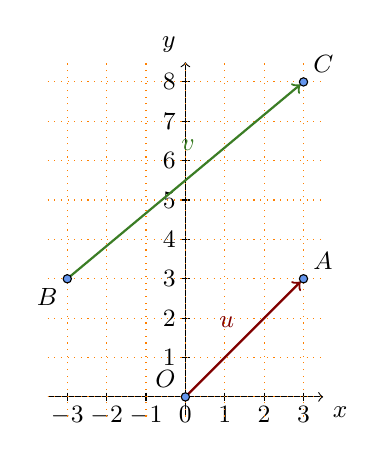
\begin{tikzpicture}[x=5mm,y=5mm, font=\small]

  \begin{scope}[->]
    \draw (-3.5,0) -- (3.5,0) node [below right] {$x$};
    \draw (0,-.5) -- (0,8.5) node[above left] {$y$};
  \end{scope}

  \foreach \x in {-3,-2, ..., 3}{
    \node[below] at (\x, 0) {$\x$};
    \draw (\x,1.5pt) -- (\x,-1.5pt);}
  \foreach \y in {1, 2, ..., 8}{
    \node[left] at (0, \y) {$\y$};
    \draw (1.5pt,\y) -- (-1.5pt,\y);}
  \draw [dotted, orange, step=1](-3.5,-.5) grid (3.5,8.5);

  \begin{scope}[thick, ->,shorten >=1.5pt]
	\draw[Maroon] (0,0) node[above left] at (1.5,1.5) {$u$} -- (3,3);  
	\draw[OliveGreen](-3,3) node[above left] at (.5,6) {$v$}-- (3,8);
      \end{scope}
 
\begin{scope}[fill=CornflowerBlue, draw=black]
\filldraw (0,0) circle (1.5pt)node [above left]{$O$};
\filldraw (3,3) circle (1.5pt)node [above right]{$A$};
\filldraw (-3,3) circle (1.5pt)node [below left]{$B$};
\filldraw (3,8) circle (1.5pt) node [above right]{$C$};
\end{scope}

\end{tikzpicture}
%  \caption{Es. 26.14.}\label{fig:G.10}
%  \end{minipage}
% \end{figure}
% \end{inaccessibleblock}

\begin{multicols}{2}
\begin{esercizio}
\label{ese:G.14}
La proiezione~$AH$ è di~$2$ metri. Determinate la misura 
del segmento ``proiettante'' $AB$ nei seguenti casi:~${\hat{\alpha}}=28\grado$
${\hat{\alpha}}=45\grado$ ${\hat{\alpha}}=60\grado$ ${\hat{\alpha}}=88\grado$ 
(con l'approssimazione alla quarta cifra decimale).
\begin{center}
 % (c) 2012 Dimitrios Vrettos - d.vrettos@gmail.com
% (c) 2015 Daniele Zambelli - daniele.zambelli@gmail.com

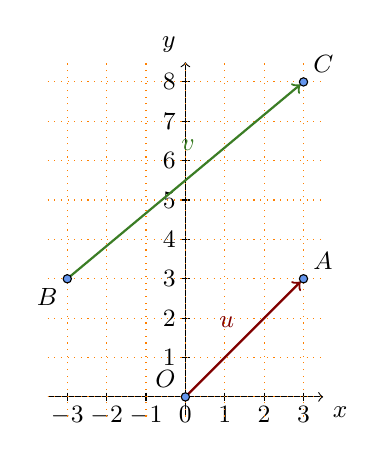
\begin{tikzpicture}[x=5mm,y=5mm, font=\small]

  \begin{scope}[->]
    \draw (-3.5,0) -- (3.5,0) node [below right] {$x$};
    \draw (0,-.5) -- (0,8.5) node[above left] {$y$};
  \end{scope}

  \foreach \x in {-3,-2, ..., 3}{
    \node[below] at (\x, 0) {$\x$};
    \draw (\x,1.5pt) -- (\x,-1.5pt);}
  \foreach \y in {1, 2, ..., 8}{
    \node[left] at (0, \y) {$\y$};
    \draw (1.5pt,\y) -- (-1.5pt,\y);}
  \draw [dotted, orange, step=1](-3.5,-.5) grid (3.5,8.5);

  \begin{scope}[thick, ->,shorten >=1.5pt]
	\draw[Maroon] (0,0) node[above left] at (1.5,1.5) {$u$} -- (3,3);  
	\draw[OliveGreen](-3,3) node[above left] at (.5,6) {$v$}-- (3,8);
      \end{scope}
 
\begin{scope}[fill=CornflowerBlue, draw=black]
\filldraw (0,0) circle (1.5pt)node [above left]{$O$};
\filldraw (3,3) circle (1.5pt)node [above right]{$A$};
\filldraw (-3,3) circle (1.5pt)node [below left]{$B$};
\filldraw (3,8) circle (1.5pt) node [above right]{$C$};
\end{scope}

\end{tikzpicture}
\end{center}
\end{esercizio}

\begin{esercizio}
\label{ese:G.15}
In un triangolo rettangolo conoscendo il coseno dell'angolo 
acuto~$\hat{\alpha}=0,3$ calcola~$\sin \alpha$ e~$\tan \alpha$
Calcola, inoltre, il valore dell'angolo acuto~$\hat{\alpha}$ in gradi e decimali 
di grado.
\end{esercizio}

\begin{esercizio}
\label{ese:G.16}
In un triangolo rettangolo di angolo acuto~$x$, calcola~$\cos x$, $\tan x$ 
e~$x$ sapendo che~$\sin x=0,2$
\end{esercizio}

\begin{esercizio}
\label{ese:G.17}
In un triangolo rettangolo di angolo acuto~$x$, calcola~$\sin x$, $\cos x$ 
e~$x$ sapendo che~$\tan x =1,5$
\end{esercizio}

\begin{esercizio}
\label{ese:G.18}
In un triangolo rettangolo conoscendo il coseno dell'angolo 
acuto~$\hat{\alpha}$, $\cos \alpha = 0,7$ calcola~$\sin \alpha$ e~$\tan \alpha$
Calcola, inoltre, il valore dell'angolo acuto~$\hat{\alpha}$ in gradi e decimali 
di grado.
\end{esercizio}

\begin{esercizio}
\label{ese:G.19}
Trova area e perimetro del triangolo rettangolo~$ABC$ retto in~$A$ sapendo 
che~$AB=50\unit{cm}$
\end{esercizio}

\begin{esercizio}
\label{ese:G.20}
Risolvi il triangolo rettangolo che ha un cateto di~$25\unit{cm}$ e il seno 
dell'angolo ad esso adiacente pari a~$0,28$
\end{esercizio}

\begin{esercizio}
\label{ese:G.21}
In un triangolo rettangolo conoscendo il coseno dell'angolo 
acuto~$\hat{\alpha}$, $\cos \alpha = 0,2$ calcola~$\sin \alpha$ e
$\tan \alpha$ Calcola, inoltre, la misura dei restanti lati sapendo che il 
cateto opposto ad~$\hat{\alpha}$ misura~$66\unit{cm}$
\end{esercizio}
\end{multicols}

% \subsubsection*{G.7 - Risoluzione di un triangolo qualsiasi con triangoli 
% rettangoli}
\numnameref{sec:trigo_altritriangoli}

\begin{esercizio}
\label{ese:G.22}
Risolvi il triangolo acutangolo~$ABC$ nei seguenti casi.
\begin{multicols}{2}
\begin{enumeratea}
\item ${CH}=20\unit{cm}$,\, $\hat{\alpha} =45\grado$,\,$\hat{\beta} 
=62\grado~20'$
\item ${AC}=20\unit{cm}$,\, $\hat{\alpha} =60\grado$,\,$\hat{\beta} =35\grado$
\item ${BH}=12\unit{cm}$,\, $\hat{\alpha} =35\grado$,\,$\hat{\beta} 
=40\grado~30'$
\item ${AH}=22,25\unit{cm}$,\, $\hat{\alpha} =20\grado$,\,$\hat{\beta} 
=65\grado$
\item ${CH}=10\unit{cm}$,\, $\hat{\alpha} =42\grado$,\,$\hat{\beta} =53\grado$
\end{enumeratea}
\end{multicols}
\end{esercizio}

\begin{esercizio}
\label{ese:G.23}
In riferimento alla seguente figura risolvi il triangolo~$ABC$, conoscendo gli 
elementi indicati.
\begin{center}
\begin{inaccessibleblock}[Triangolo ottusangolo con l'altezza relativa a uno
dei lati più corti.]
 % (c) 2012 Dimitrios Vrettos - d.vrettos@gmail.com

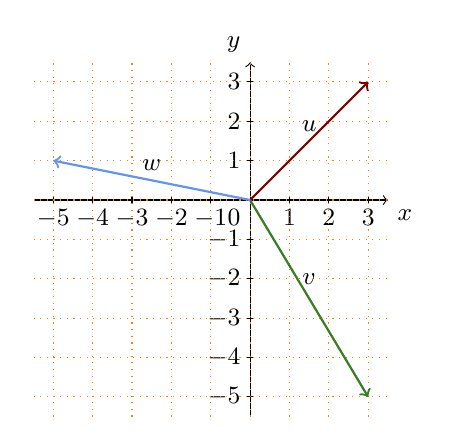
\begin{tikzpicture}[x=5mm,y=5mm, font=\small]

  \begin{scope}[->]
    \draw (-5.5,0) -- (3.5,0) node [below right] {$x$};
    \draw (0,-5.5) -- (0,3.5) node[above left] {$y$};
  \end{scope}

  \foreach \x/\xtext in {-5/-5,-4/-4,-3/-3,-2/-2,-1/-1,1/1,2/2,3/3}{
    \node[below] at (\x,0) {$\xtext$};
    \draw (\x,1.5pt) -- (\x,-1.5pt);}
  \foreach \y/\ytext in {-5/-5,-4/-4,-3/-3,-2/-2,-1/-1,1/1,2/2,3/3}{
    \node[left] at (0,\y) {$\ytext$};
    \draw (1.5pt,\y) -- (-1.5pt,\y);}
  \node[below left] at (0,0) {$0$};

  \begin{scope}[dotted, orange, step=5mm]
    \draw (-5.5,-5.5) grid (3.5,3.5);
  \end{scope}

  \begin{scope}[thick, ->]
	\draw[Maroon] (0,0) -- (3,3);  
	\draw[OliveGreen](0,0) -- (3,-5);
	\draw[CornflowerBlue] (0,0) -- (-5,1);
      \end{scope}
 
\node[above] at (1.5,1.5) {$u$};
\node[above] at (1.5,-2.4) {$v$};
\node[above] at (-2.5,.5) {$w$};
\end{tikzpicture}
\end{inaccessibleblock}
\end{center}
\begin{multicols}{2}
 \begin{enumeratea}
\item ${AB}=2\unit{cm}$,\, ${BC}=6\unit{cm}$,\,$\hat{\beta} =30\grado$
\item ${CH}=50\unit{cm}$,\, ${AB}=76\unit{cm}$,\,$\hat{\alpha} =120\grado$
\end{enumeratea}
\end{multicols}
\end{esercizio}

\begin{multicols}{2}
\begin{esercizio}
\label{ese:G.24}
Risolvere un triangolo isoscele nota la base$=4\sqrt{2}\unit{cm}$ e 
l'$\Area=32\unit{cm^2}$
\end{esercizio}

\begin{esercizio}
\label{ese:G.25}
Un triangolo isoscele ha l'altezza relativa alla base lunga~$120\unit{cm}$ e il 
seno dell'angolo alla base è uguale a~$\frac{2}{3}$
Calcola perimetro e area del triangolo.
\end{esercizio}
\end{multicols}

\newpage

% \paragraph{Quadrilateri}
\numnameref{subsec:trigo_quadrilatei}

\begin{multicols}{2}
 \begin{esercizio}
\label{ese:G.26}
Nel trapezio~$ABCD$ isoscele sulla base maggiore~$AB$, la base minore 
misura~$30\unit{cm}$, i lati obliqui~$20\unit{cm}$
e il seno degli angoli acuti è~$0,6$ Trova la misura del perimetro e dell'area.
\end{esercizio}

\begin{esercizio}
\label{ese:G.27}
Trova l'area di un rombo di perimetro~$120\unit{cm}$ e con angolo ottuso pari 
a~$100\grado$
\end{esercizio}

\begin{esercizio}
\label{ese:G.28}
Trova la misura del lato e dell'altezza del rombo con diagonale maggiore 
di~$20\unit{cm}$ e con uno dei due angoli acuti di~$30\grado$
\end{esercizio}

\begin{esercizio}
\label{ese:G.29}
Trova le due altezze del parallelogramma di lati~$10\unit{cm}$ e~$15\unit{cm}$ e 
con i due angoli acuti di~$20\grado$
\end{esercizio}

\begin{esercizio}
\label{ese:G.30}
Trova l'area di un parallelogramma sapendo che i lati sono 
lunghi~$12,5\unit{cm}$ e~$7,8\unit{cm}$ e l'angolo tra essi compreso 
è~$44\grado~30'$
\end{esercizio}

\begin{esercizio}
\label{ese:G.31}
Calcola l'area di un rombo sapendo che il lato è~$12\unit{cm}$ e l'angolo ottuso 
di~$120\grado$
\end{esercizio}

\begin{esercizio}
\label{ese:G.32}
Calcola l'area e il perimetro di un rettangolo sapendo che le sue diagonali 
misurano~$10\unit{cm}$
e che gli angoli che esse formano con la base sono di~$35\grado30'$
\end{esercizio}

\begin{esercizio}
\label{ese:G.33}
L'area di un trapezio isoscele è~$28\unit{cm^2}$ e il suo perimetro 
è~$24\unit{cm}$ Determina gli angoli del trapezio,
sapendo che la sua altezza è~$4\unit{cm}$
\end{esercizio}
\end{multicols}

% \paragraph{Applicazioni alla topografia}
\numnameref{subsec:trigo_applicazioni}

\begin{multicols}{2}
 \begin{esercizio}
\label{ese:G.34}
Risolvere il quadrilatero~$ABCD$ sapendo che~${AB}=8,01\unit{m}$,
${BC}=5,54\unit{m}$, ${CD}=4,63\unit{m}$, $\widehat{BAD}=40\grado$, 
$\widehat{ADC}=50\grado$
\end{esercizio}

\begin{esercizio}
\label{ese:G.35}
Risolvere il quadrilatero~$ABCD$ sapendo che  ${AB}=5,8\unit{m}$, 
${BC}=6,24\unit{m}$,
${CD}=12,81\unit{m}$, $\widehat{BAD}=45\grado$, $\widehat{ADC}=65\grado$
(attenzione: in questo problema~${CD}>{AB}$, quindi la figura va disegnata 
diversamente).
\end{esercizio}

%  \begin{esercizio}
% \label{ese:G.36}
% Risolvere il quadrilatero~$ABCD$ della figura sapendo che~${AB}=33,28\unit{m}$, 
% ${CD}=59,7\unit{m}$,
% $\widehat{BAD}=102\grado$, $\widehat{DCB}=63\grado$, $\widehat{ADC}=72\grado$
% 
% \emph{Suggerimento}: tracciare i segmenti come nella figura sotto e osservare i 
% triangoli e il rettangolo che si forma.
% \begin{center}
% \begin{inaccessibleblock}[Quadrilatero suddiviso in rettangoli e 
% triangoli rettangoli.]
%  % (c) 2012 Dimitrios Vrettos - d.vrettos@gmail.com

\begin{tikzpicture}[x=10mm,y=10mm, font=\small]
\tkzDefPoint(0,0){A}
\tkzDefShiftPoint[A](102:3.328){B}
\tkzDefShiftPoint[A](0:3){D}
\tkzDefShiftPoint[D](108:5.97){C}

\tkzMarkAngle[fill=LimeGreen, draw=black, size=.4](D,A,B)
\tkzMarkAngle[fill=LimeGreen, draw=black, size=.4](C,D,A)
\tkzMarkAngle[fill=LimeGreen, draw=black, size=.5](B,C,D)

\tkzDefPointBy[projection=onto A--D](C) 
\tkzGetPoint{E}

\tkzDefPointBy[projection=onto A--D](B) 
\tkzGetPoint{F}

\tkzDefPointBy[projection=onto C--E](B) 
\tkzGetPoint{G}

\tkzDrawLine[add=0 and 0, thin](A,B)
\tkzDrawLine[add=0 and 0, thin](A,D)
\tkzDrawLine[add=0 and 0, thin](D,C)
\tkzDrawLine[add=0 and 0, thin](C,B)

\tkzDrawLine[add=0 and 0, thin,dashed](B,F)
\tkzDrawLine[add=0 and 0, thin,dashed](B,G)
\tkzDrawLine[add=0 and 0, thin,dashed](A,F)
\tkzDrawLine[add=0 and 0, thin,dashed](C,E)

\tkzLabelPoints[below](A,F,D,E)
\tkzLabelPoints[above](C)
\tkzLabelPoints[left](B)
\tkzLabelPoints[right](G)
\tkzDrawPoints[color=CornflowerBlue](A,B,C,D,F,E,G)

\end{tikzpicture}
% \end{inaccessibleblock}
% \end{center}
% \end{esercizio}
% \end{multicols}
% \newpage
% \paragraph{Applicazioni alla fisica}
% \begin{multicols}{2}
\begin{esercizio}
\label{ese:G.37}
Un vettore velocità~$\vec{v}$ ha modulo $12\unit{cm/sec}$ Posto su un piano 
cartesiano $O_{xy}$, forma un angolo di $30\grado$ con
l'asse delle ascisse. Trova le componenti di~$\vec{v}$, $\vec{v}_x$ 
e~$\vec{v}_y$ sugli assi.
\end{esercizio}

\begin{esercizio}
\label{ese:G.38}
Un piano inclinato forma col piano d'appoggio un angolo di~$16\grado$ Determina 
la forza non equilibrata che farà scivolare un corpo di
$12\unit{kg}$ lungo un piano inclinato.
\end{esercizio}

\begin{esercizio}
\label{ese:G.39}
Calcola la forza necessaria per mantenere in stato di quiete un corpo del peso 
di~$25\unit{kg}$ su un piano inclinato con
la pendenza di~$20\grado~15'$
\end{esercizio}

\begin{esercizio}
\label{ese:G.40}
Calcola la lunghezza del vettore~$\vec{v}(3;4)$ e gli angoli che esso forma con 
gli assi cartesiani.
Calcola inoltre l'equazione della retta che ha la stessa direzione del 
vettore~$\vec{v}$ e passa per il punto~$A(0;1)$
\end{esercizio}

\begin{esercizio}
\label{ese:G.41}
Un aereo viaggia da~$A$ a~$B$ che distano~$1000\unit{km}$, in assenza di vento 
l'aereo impiega un'ora per effettuare il percorso.
Quel giorno però sulla tratta~$AB$ soffia un vento costante di 
intensità~$100\unit{km/ora}$ e direzione di~$240$ gradi
rispetto alla direzione~$AB$ Calcola il tempo impiegato e l'angolo di rotta 
necessario per mantenere la direzione~$AB$
\end{esercizio}


\begin{esercizio}[\Ast]
\label{ese:G.42}
Parto da una località~$A$ ai piedi di una collina per raggiungere una 
località~$B$ che si trova nell'altro versante della collina,
alla stessa quota di~$A$ Per fare questo percorro per~$467\unit{m}$ una dritta 
mulattiera che sale con pendenza costante di~$30\grado$
Poi percorro in discesa~$300\unit{m}$ lungo un dritto sentiero scalinato con 
pendenza costante di~$50\grado$ e giungo alla località~$B$
Quanto sarebbe lungo un tunnel che congiungesse~$A$ con~$B$?
\begin{center}
\begin{inaccessibleblock}[Montagna con una pendenza, da una parte di 30 e 
dall'altra di 50 gradi.]
 % (c) 2012 Dimitrios Vrettos - d.vrettos@gmail.com

\begin{tikzpicture}[x=10mm,y=10mm, font=\small]
 \tkzDefPoint(0,0){A}
 \tkzDefShiftPoint[A](30:4.67){C}
 \tkzDefShiftPoint[A](0:5.97){B}

 \tkzMarkAngle[fill=LimeGreen, draw=black, size=.4](B,A,C)
 \tkzMarkAngle[fill=LimeGreen, draw=black, size=.4](C,B,A)

\tkzDrawLine[add=0 and 0, thin,dashed](A,B)
\tkzDrawLine[add=0 and 0, thin](A,C)
\tkzDrawLine[add=0 and 0, thin](B,C)

 \tkzLabelPoints[below](A,B)
\tkzLabelAngle[](B,A,C){$30^\circ$}
\tkzLabelAngle[](C,B,A){$50^\circ$}
 \tkzDrawPoints[color=CornflowerBlue](A,B,C)
 
\end{tikzpicture}
\end{inaccessibleblock}
\end{center}
\hfill [$597,27\unit{m}$]
\end{esercizio}

\begin{esercizio}[\Ast]
\label{ese:G.43}
Per andare da una località~$A$ ad una località~$B$ poste in una pianura mi 
muovo, in aereo e sempre alla stessa quota, di~$20\unit{Km}$
nella direzione che forma un angolo di~$20\grado$ rispetto alla direzione~$AB$ 
Poi, per riavvicinarmi alla congiungente~$AB$,
mi muovo di~$35\unit{Km}$ lungo la direzione che forma un angolo di~$60\grado$ 
rispetto ad~$AB$ Infine percorro~$24,7\unit{Km}$
nella direzione che forma un angolo di~$71,82\grado$ (ovvero~$71\grado~49' 
12''$) rispetto ad~$AB$ giungendo finalmente sopra a~$B$
Quanto dista~$A$ da~$B$?

\emph{Attenzione}: sulla calcolatrice si può digitare sia~$\cos 71,82\grado$ 
che~$\cos 71\grado~49' 12''$ purché la calcolatrice sia
impostata con i gradi (D o Deg sul display; G o Grad indica un'altra unità di 
misura!).

\begin{center}
\begin{inaccessibleblock}[Tre segmenti consecutivi che formano con 
l'orizzontale rispettivamente angoli di 20, -60 e 71,82 gradi.]
 % (c) 2012 Dimitrios Vrettos - d.vrettos@gmail.com

\begin{tikzpicture}[x=10mm,y=10mm, font=\small]
 \tkzDefPoint(0,0){A}
 \tkzDefShiftPoint[A](20:2){C}
 \tkzDefShiftPoint[C](300:3.5){D}
 \tkzDefShiftPoint[C](0:2){E}
 \tkzDefShiftPoint[D](0:1){F}
 \tkzDefShiftPoint[A](0:4.4){B}

  \tkzMarkAngle[fill=LimeGreen, draw=black, size=.5](B,A,C)
 \tkzMarkAngle[fill=LimeGreen, draw=black, size=.4](D,C,E)
 \tkzMarkAngle[fill=LimeGreen, draw=black, size=.4](F,D,B)

\tkzDrawLine[add=0 and 0, thin](A,C)
\tkzDrawLine[add=0 and 0, thin](C,D)
\tkzDrawLine[add=0 and 0, thin](B,D)
 
\tkzLabelPoints[below](A)
 \tkzLabelPoints[above](B)
\tkzLabelAngle(B,A,C){$20^\circ$}
\tkzLabelAngle[pos=.8](D,C,E){$60^\circ$}
\tkzLabelAngle[pos=.8](F,D,B){$71.82^\circ$}
 \tkzDrawPoints[color=CornflowerBlue](A,B,C,D)
 
\end{tikzpicture}
\end{inaccessibleblock}
\end{center}
\hfill [$44\unit{Km}$]
\end{esercizio}

\end{multicols}

\begin{esercizio}[\Ast]
\label{ese:G.44}
Sono in barca a vela e parto dalla boa~$B_i$ per raggiungere la boa~$B_f$ Inizio 
la navigazione percorrendo un tratto lungo~$1\unit{km}$
nella direzione che forma un angolo di~$10\grado$ rispetto al tratto~$B_i B_f$ 
Poi viro per riavvicinarmi a~$B_i B_f$ e percorro un tratto
di~$2\unit{Km}$ nella direzione che forma un angolo di~$10\grado$ rispetto 
a~$B_i B_f$ Ripeto la virata di~$10\grado$ per
riavvicinarmi alla congiungente~$B_i B_f$ e percorro di nuovo~$2\unit{km}$ 
Faccio un'ultima virata di~$10\grado$ che, percorrendo~$1\unit{Km}$,
mi porta esattamente a~$B_f$ Quanto dista~$B_i$ da~$B_f$?
% \newpage
\begin{center}
\begin{inaccessibleblock}[Percorso a zig zag in barca a vela con angoli
alternati di 10 e -10 gradi.]
 % (c) 2012 Dimitrios Vrettos - d.vrettos@gmail.com

\begin{tikzpicture}[x=10mm,y=10mm, font=\small]
 \tkzDefPoint(0,0){B_i}
 \tkzDefShiftPoint[B_i](10:2){A}
 \tkzDefShiftPoint[A](350:4){C}
 \tkzDefShiftPoint[A](0:1){A'}
 \tkzDefShiftPoint[C](0:1){C'}
 \tkzDefShiftPoint[C](10:4){D}
 \tkzDefShiftPoint[D](0:1){D'}
 \tkzDefShiftPoint[D](350:2){B_f}

 \tkzMarkAngle[fill=LimeGreen, draw=black, size=1](B_f,B_i,A)
 \tkzMarkAngle[fill=LimeGreen, draw=black, size=1](C,A,A')
 \tkzMarkAngle[fill=LimeGreen, draw=black, size=1](C',C,D)
 \tkzMarkAngle[fill=LimeGreen, draw=black](B_f,D,D')

 \tkzDrawLine[add=0 and 0, thin](B_i, A)
 \tkzDrawLine[add=0 and 0, thin](C, A)
 \tkzDrawLine[add=0 and 0, thin](C,D)
 \tkzDrawLine[add=0 and 0, thin](B_f,D)
\tkzDrawLine[add=0 and 0, thin,dotted](B_f,B_i)

 \tkzLabelPoints[below](B_i, B_f)

 \tkzLabelAngle[below](B_f,B_i,A){$10^\circ$} \tkzLabelAngle[above](A',A,C){$10^\circ$}
\tkzLabelAngle[below](D,C,C'){$10^\circ$}
\tkzLabelAngle[above](D',D,B_f){$10^\circ$}
 \tkzDrawPoints[color=CornflowerBlue](B_i,A,C,D,B_f)
 
\end{tikzpicture}
\end{inaccessibleblock}
\end{center}
\hfill [$5,91\unit{Km}$]
\end{esercizio}

\begin{esercizio}[\Ast]
\label{ese:G.45}
Faccio una dritta salita che separa due località distanti in linea 
d'aria~$5\unit{Km}$ Se la pendenza della salita è di~$8\grado$ costanti,
qual'è (in metri) la differenza di quota delle due località?
\hfill [$695,87\unit{m}$]
\end{esercizio}

\begin{esercizio}[\Ast]
\label{ese:G.46}
In barca a vela mi muovo dalla boa~$B_i$ alla boa~$B_f$ facendo un percorso a 
zig zag in cui ciascun tratto forma angoli di~$25\grado$
rispetto al segmento~$B_i B_f$ Dopo aver navigato per quattro tratti, di cui il 
primo lungo~$4\unit{Km}$ e i restanti~$8\unit{Km}$,
quanto percorso è stato fatto nella direzione~$B_i B_f$?
\begin{center}
\begin{inaccessibleblock}[Percorso a zig zag in barca a vela con angoli
alternati di 25 e -25 gradi.]
 % (c) 2012 Dimitrios Vrettos - d.vrettos@gmail.com

\begin{tikzpicture}[x=9mm,y=9mm, font=\small]
 \tkzDefPoint(0,0){B_i}
 \tkzDefShiftPoint[B_i](25:2){A}
 \tkzDefShiftPoint[A](335:4){C}
 \tkzDefShiftPoint[A](0:1){A'}
 \tkzDefShiftPoint[C](0:1){C'}
 \tkzDefShiftPoint[C](25:4){D}
 \tkzDefShiftPoint[D](0:1){D'}
\tkzDefShiftPoint[D](335:4){D''} 
\tkzDefShiftPoint[D''](25:2){B_f}

 \tkzMarkAngle[fill=LimeGreen, draw=black, size=1](B_f,B_i,A)
 \tkzMarkAngle[fill=LimeGreen, draw=black, size=1](C,A,A')
 \tkzMarkAngle[fill=LimeGreen, draw=black, size=1](C',C,D)
 \tkzMarkAngle[fill=LimeGreen, draw=black](D'',D,D')

 \tkzDrawLine[add=0 and 0, thin](B_i, A)
 \tkzDrawLine[add=0 and 0, thin](C, A)
 \tkzDrawLine[add=0 and 0, thin](C,D)
 \tkzDrawLine[add=0 and 0, thin](D,D'')

\tkzDrawLine[add=0 and 0, thin,dotted](B_f,B_i)

 \tkzLabelPoints[below](B_i, B_f)

 \tkzLabelAngle[pos=1.3](B_f,B_i,A){$25^\circ$} \tkzLabelAngle[pos=1.3](A',A,C){$25^\circ$}
\tkzLabelAngle[pos=1.3](D,C,C'){$25^\circ$}
\tkzLabelAngle[pos=1.3](D',D,B_f){$25^\circ$}
 \tkzDrawPoints[color=CornflowerBlue](B_i,A,C,D,D'',B_f)
 
\end{tikzpicture}
\end{inaccessibleblock}
\end{center}
\hfill [$25,38\unit{Km}$]
\end{esercizio}

\begin{multicols}{2}

\begin{esercizio}[\Ast]
\label{ese:G.47}
Devo stendere un cavo dell'impianto parafulmine lungo il tetto e la parete di 
una casa facendolo poi affondare nel terreno per~$10\unit{m}$
Quale deve essere la lunghezza minima del cavo sapendo che (vedi figura) il 
parafulmine è posto sul punto più alto del tetto e la casa è
composta da un pian terreno ed un primo piano completi di altezza standard 
(cioè~$3\unit{m}$ ciascuno), è larga~$9\unit{m}$,
ha un tetto ad una falda inclinato di~$16\grado$? (La figura rappresenta la 
sezione della casa).
\begin{center}
\begin{inaccessibleblock}[Sezione di una casetta con un parafulmine.]
 % (c) 2012 Dimitrios Vrettos - d.vrettos@gmail.com

\begin{tikzpicture}[x=10mm,y=10mm, font=\small]
\coordinate (A) at (0,0);
\coordinate (B) at ($(A) +(0:3)$);
 \coordinate (C) at ($(A) +(90:2)$);
\coordinate (D) at ($(C) +(16:3.12)$);

\draw (A) -- (C) -- (D) --(B)--(A);

\node (a) at (0,0) {};
\node[ground,anchor=center] (g) {};
\draw (a.south) -- (g);

\draw (D) to[short, -o] (3,3);

\end{tikzpicture}
\end{inaccessibleblock}
\end{center}
\hfill [$25,36\unit{m}$]
\end{esercizio}


 \begin{esercizio}[\Ast]
\label{ese:G.48}
Percorro una salita rettilinea con pendenza di~$10\grado$ partendo da una 
località~$A$ posta a~$400\unit{m}$ d'altezza e arrivando ad
una località~$B$ posta a quota~$700\unit{m}$ Quanto dista~$A$ da~$B$?
\hfill [$2.303,50\unit{m}$]
\end{esercizio}

\begin{esercizio}[\Ast]
\label{ese:G.49}
Dalla cima di un palco alto~$1,30\unit{m}$ un tizio alto~$1,70\unit{m}$ osserva 
la punta di un obelisco sotto un angolo di~$40\grado$
Con un laser misura la distanza tra il suo occhio e la cima dell'obelisco e 
trova~$74\unit{m}$ Quanto è alto l'obelisco?

\emph{Attenzione}: osservare un oggetto sotto un angolo~$\hat{\alpha}$ significa 
che la retta congiungente il nostro occhio con l'oggetto osservato
forma un angolo~$\hat{\alpha}$ con una retta orizzontale.
\hfill [${59,68\unit{m}}$]
\end{esercizio}

\begin{esercizio}[\Ast]
\label{ese:G.50}
Una mansarda è alta~$5\unit{m}$ e la sua sezione è un triangolo isoscele con 
angoli alla base di~$50\grado$ Quant'è larga la mansarda?
(Ricorrere solo alla trigonometria; usare sia la formula diretta della 
proiezione sia la formula inversa.)
\hfill [$8,39\unit{m}$]
\end{esercizio}
\end{multicols}

\paragraph{Problemi sulle forze}
% \numnameref{}

\begin{multicols}{2}
 \begin{esercizio}[\Ast]
\label{ese:G.51}
Per trainare un vagone fermo su un binario uso un locomotore posto in un binario 
parallelo ed un cavo in acciaio che, in trazione,
forma un angolo di~$22\grado$ rispetto ai binari. Sapendo che l'intensità della 
forza di trazione lungo il cavo è di~$35.000\unit{N}$,
qual è il modulo della forza che fa muovere il vagone?
\hfill [$32.451\unit{N}$]
\end{esercizio}

\begin{esercizio}[\Ast]
\label{ese:G.52}
Per estrarre un manicotto (cioè un cilindro cavo) incastrato in un paletto 
esercito una forza di~$150\unit{N}$ tramite un filo che,
teso durante la trazione, forma un angolo di~$20\grado$ rispetto all'asse del 
paletto. Di che intensità è la forza che mi sarebbe
bastato applicare per estrarre il manicotto se l'avessi esercitata lungo l'asse 
del paletto?
\hfill [$140,95\unit{N}$]
\end{esercizio}

\begin{esercizio}[\Ast]
\label{ese:G.53}
Per trainare un vagone lungo un binario devo esercitare una forza minima 
di~$20.000\unit{N}$ lungo la direzione del binario.
Qual è l'intensità minima della forza che devo esercitare sul vagone perché si 
sposti sapendo che la direzione della forza che posso
applicare forma un angolo di~$40\grado$ con la direzione del binario?
\hfill [$26.108,95\unit{N}$]
\end{esercizio}

\begin{esercizio}[\Ast]
\label{ese:G.54}
Una mansarda è alta~$5\unit{m}$ e la sua sezione è un triangolo isoscele con 
angoli alla base di~$50\grado$ Quant'è larga la mansarda?
\hfill [$8,39\unit{m}$]
\end{esercizio}

\begin{esercizio}
\label{ese:G.55}
Come si può misurare l'altezza di un edificio, senza salirvi in cima, disponendo 
di un metro a nastro e di un teodolite in grado di
misurare a vista angoli sul piano verticale?
\end{esercizio}

\begin{esercizio}[\Ast]
\label{ese:G.56}
Dal tetto di una casa alta~$9\unit{m}$ un bimbo alto~1m osserva sotto un angolo 
di~$6\grado$ la punta di un obelisco che,
in base ad una mappa, dista~$232\unit{m}$ dalla casa. Quanto è alto l'obelisco?
\hfill [$34,38\unit{m}$]
\end{esercizio}

\begin{esercizio}[\Ast]
\label{ese:G.57}
Nella capriata di una cattedrale la cui sezione è un triangolo isoscele, la 
lunghezza della catena (cioè della base del triangolo isoscele) è di
$50\unit{m}$ e il tetto è inclinato di~$15\grado$ rispetto al pavimento. Quanto 
è alta la capriata?
\hfill [$6,70\unit{m}$]
\end{esercizio}

\begin{esercizio}[\Ast]
\label{ese:G.58}
La grande piramide di Cheope ha una base quadrata larga circa~$230\unit{m}$ 
Sapendo che le pareti sono inclinate di circa~$52\grado$,
quanto è alta la piramide?

\emph{Attenzione}: l'inclinazione cui si fa riferimento è quella delle apoteme 
delle facce laterali rispetto al terreno.
\hfill [$147\unit{m}$]
\end{esercizio}

\begin{esercizio}[\Ast]
\label{ese:G.59}
Si attribuisce all'architetto dell'Antico Egitto \emph{Imhotep} l'intuizione che 
l'inclinazione delle pareti di una piramide non deve superare
i~$53\grado$ per evitare problemi di slittamento dei blocchi del rivestimento 
sotto l'effetto di un sisma. Ammesso di usare
l'inclinazione massima, quanto deve essere larga una piramide che debba 
raggiungere l'altezza di~$70\unit{m}$?
E se, per sicurezza, si volesse usare un'inclinazione di~45°?

\emph{Suggerimento}: questo problema si può risolvere usando l'angolo 
complementare a quello assegnato.
\hfill [$105,50\unit{m}$\,$140\unit{m}$]
\end{esercizio}

\begin{esercizio}[\Ast]
\label{ese:G.60}
Una mansarda avente per sezione un triangolo isoscele è alta~$4\unit{m}$ e 
larga~$15\unit{m}$ Qual è l'inclinazione del tetto?
\hfill [$28\grado$]
\end{esercizio}

\begin{esercizio}[\Ast]
\label{ese:G.61}
La piramide di Meidum, così come modificata sotto Snefru, era 
alta~$91,7\unit{m}$ e larga~$144\unit{m}$
Quanto erano inclinate rispetto al terreno le (apoteme delle) sue facce?
\hfill [$51,86\grado$]
\end{esercizio}

\begin{esercizio}[\Ast]
\label{ese:G.62}
Dall'Avenue des Champs-Élysées osservo la sommità dell'Arco di Trionfo 
napoleonico sotto un angolo di~$36\grado$.
Sapendo che l'Arco è alto~$50\unit{m}$ quanto disto dalla sua base? Se mi trovo 
a~$1,2\unit{Km}$ dalla sua base,
sotto che angolo ne osservo la sommità?
\hfill [$68,82\unit{m}$\,$2,39\grado$]
\end{esercizio}

\begin{esercizio}[\Ast]
\label{ese:G.63}
Devo stendere un tirante che si aggancia a terra e ad un palo, ai~$\frac{3}{5}$ 
della sua altezza.
Sapendo che il palo è alto~$3,34\unit{m}$ e che il cavo si aggancia al terreno 
a~$3\unit{m}$ dalla sua base,
che angolo forma il tirante rispetto al terreno?
\hfill [$33,74\grado$]
\end{esercizio}

\begin{esercizio}[\Ast]
\label{ese:G.64}
Su un cartello stradale vediamo l'indicazione di una salita del~$10\%$ Sapendo 
che questo significa che ogni~$100\unit{m}$
in orizzontale se ne percorrono~$10$ in verticale, calcola l'inclinazione in 
gradi della strada. È possibile superare salite del~$100\%$?
\hfill [$5,71\grado$]
\end{esercizio}

\begin{esercizio}[\Ast]
\label{ese:G.65}
Una capriata ha una catena di~$32\unit{m}$ ed è alta~$8,9\unit{m}$ Qual è 
l'inclinazione dei suoi puntoni?

\emph{Attenzione}: la capriata è la struttura per le coperture a 
{\textquotedbl}capanna{\textquotedbl}; le travi che la costituiscono
formano un triangolo isoscele; la catena è la trave di base, i puntoni sono le 
travi oblique.
\hfill [$29,08\grado$]
\end{esercizio}

\begin{esercizio}[\Ast]
\label{ese:G.66}
La facciata di un tempio greco ha un basamento largo~$22\unit{m}$ e 
alto~$3\unit{m}$, colonne alte~$7,40\unit{m}$ e il frontone,
largo quanto il basamento, ha falde inclinate di~$15\grado$ Quanto è alto il 
punto più elevato del tempio?
Volendo fargli raggiungere l'altezza di~$14\unit{m}$ quale inclinazione 
bisognerebbe dare ai lati obliqui del frontone?
\hfill [$13,35\unit{m}$\,$18,12\grado$]
\end{esercizio}

\begin{esercizio}[\Ast]
\label{ese:G.67}
Dall'alto di una rampa lunga~$300\unit{m}$ misuro la distanza dalla sommità di 
una torre che si eleva dalla base della rampa e arriva
alla stessa altezza della mia testa. Sapendo che la suddetta distanza 
vale~$271\unit{m}$, qual è l'inclinazione della rampa?
\hfill [$25,4\grado$]
\end{esercizio}
\end{multicols}


% \subsubsection*{G.8 - Risoluzione di un triangolo qualunque}
\numnameref{sec:trigo_triangoloqualunque}

\begin{multicols}{2}
 \begin{esercizio}
\label{ese:G.68}
Determina gli elementi incogniti di un triangolo in cui~$b=5$,\, $c=7$ 
e~${\hat{\alpha}}=74\grado$
\hfill [...]
\end{esercizio}

\begin{esercizio}
\label{ese:G.69}
In un triangolo sono noti:~$b=9$,\, ${\hat{\alpha}}=20\grado$ 
e~${\hat{\beta}}=44\grado$ Quanto vale la lunghezza~$a$?
\hfill [...]
\end{esercizio}

\begin{esercizio}
\label{ese:G.70}
In un triangolo sono noti:~$a=20$,\, $c=13$ e~${\hat{\beta}}=75\grado$ Quanto 
vale~$b$?
\hfill [...]
\end{esercizio}

\begin{esercizio}
\label{ese:G.71}
Determina l'angolo~${\hat{\beta}}$ di un triangolo in cui~$a=10\unit{Km}$,\, 
$b=8\unit{Km}$,\, $c=12\unit{Km}$
\hfill [...]
\end{esercizio}

\begin{esercizio}
\label{ese:G.72}
Determina gli elementi incogniti di un triangolo in cui~$a=12$,\, $c=15$ 
e~${\hat{\beta}}=65\grado$
\hfill [...]
\end{esercizio}

\begin{esercizio}
\label{ese:G.73}
In un triangolo sono noti:~$a= 20$,\, ${\hat{\alpha}}=35\grado$ 
e~${\hat{\beta}}=20\grado$ Quanto vale la lunghezza~$b$?
\hfill [...]
\end{esercizio}

\begin{esercizio}
\label{ese:G.74}
In un triangolo sono noti:~$b= 12$,\, $c=4$ e~${\hat{\alpha}}=40\grado$ Quanto 
vale~$a$?
\hfill [...]
\end{esercizio}
\end{multicols}
